\chapter{Physical Systems}
\label{chap:physical_systems}

\section{Hydrogen Molecule}
\label{sec:hydrogen_molecule}
The hydrogen molecule, ($ H_2 $), is the smallest molecule in chemistry. It consists of two hydrogen atoms, each with one electron. In quantum chemistry, the hydrogen molecule is often used as a benchmark for quantum algorithms. Reproducing the results of using the VQE to find the ground state energy of the hydrogen molecule is almost a textbook task in quantum computing for electronic structures. The result can also be easily benchmarked against traditional quantum chemistry methods, such as Hartree-Fock~\cite{Coleman2015}. For \quanthon, it serves as an example of how to use the software to solve electronic structure problems. 

The non-relativistic Hamiltonian for a general molecule in second quantisation is given by
\begin{equation}
	\label{eq:hamiltonian}
	H = h_{nuc} + \sum_{pq} h_{pq} a_p^\dagger a_q + \frac{1}{2} \sum_{pqrs} h_{pqrs} a_p^\dagger a_q^\dagger a_s a_r,
\end{equation}
where $ h_{nuc} $ is the interaction between nuclei and electrons, and $ h_{pq} $ and $ h_{pqrs} $ are the one and two electron integrals respectively. 
\begin{equation}
	\label{eq:elctron_integrals}
\begin{aligned}
& h_{p q}=\int d \sigma \varphi_p^*(\sigma)\left(-\frac{\nabla_{\vec{r}}^2}{2}-\sum_i \frac{Z_i}{\left|\vec{R}_i-\vec{r}\right|}\right) \varphi_q(\sigma), \\
& h_{p q r s}=\int d \sigma_1 d \sigma_2 \frac{\varphi_p^*\left(\sigma_1\right) \varphi_q^*\left(\sigma_2\right) \varphi_s\left(\sigma_1\right) \varphi_r\left(\sigma_2\right)}{\left|\vec{r}_1-\vec{r}_2\right|}, \\
& h_{n u c}=\frac{1}{2} \sum_{i \neq j} \frac{Z_i Z_j}{\left|\vec{R}_i-\vec{R}_j\right|},
\end{aligned}
\end{equation}
where $ Z_i $ is the charge of the nuclei and $ \vec{R} $ and  $\vec{r} $ are the spatial coordinates of the nuclei and electrons respectively. The functions $ \varphi $ are the one electron functions, often called spin orbitals in quantum chemistry, and are usually obtained from methods such as the Hartree Fock~\cite{Romero2019}. Fortunately, for the hydrogen molecule and many other systems, these integrals have been pre-calculated and we will be able to obtain them by using packages such as PySCF~\cite{sun2018}.

We will use the minimal basis set, namely the STO-3G basis set, which consists of three Gaussian functions for each atomic orbital~\cite{hehre1969self}. The choice of the basis set is to minimise the number of qubits required to represent the system since it is the accuracy of our VQE algorithms that is our main concern rather than capturing all the physics of the system. 

In this basis, the values we obtain for the hydrogen molecule are in Table~\ref{tab:hij} and Table~\ref{tab:hijkl}. With molecule geometry of
\begin{equation}
	\begin{aligned}
		\vec{R}_1 &= (0,0,0), \\
		\vec{R}_2 &= (0,0,0.735),
	\end{aligned}
\end{equation}
in units of angstrom (Å).

\begin{table}[h]
    \centering
    \caption{One-electron integral values of the hydrogen molecule in the STO-3G basis set.}
    \label{tab:hij}

    \begin{tabular}{c c}
        \toprule
        Integral & Values \\
        \midrule
        $h_{00} = h_{11}$ & $-1.252477$ \\
        $h_{22} = h_{33}$ & $-0.47189601$ \\
        \bottomrule
    \end{tabular}
\end{table}

\begin{table}[h]
    \centering
    \caption{Two-electron integral values for the STO-3G basis set.}
    \label{tab:hijkl}

    \begin{tabular}{c c}
        \toprule
        Integral & Values \\
        \midrule
	$h_{0000} = h_{0220} = h_{2002} = h_{2222}$ & $0.33785508$ \\
	$h_{0011} = h_{0101} = h_{0231} = h_{0321} = h_{1010} = h_{1100} = h_{1230} = h_{1320}$ & $0.09046560$ \\
	$h_{2013} = h_{2103} = h_{2233} = h_{2323} = h_{3012} = h_{3102} = h_{3232} = h_{3322}$ & $0.09046560$ \\
        $h_{0110} = h_{0330} = h_{1001} = h_{1221} = h_{2332} = h_{3003} = h_{3223}$ & $0.33229087$ \\
        $h_{1111} = h_{1331} = h_{3113} = h_{3333}$ & $0.34928686$ \\
        \bottomrule
    \end{tabular}
\end{table}


With this information, we could now perform the Jordan-Wigner transform implemented in Subsection~\ref{sub:jordan-wigner-mapper}. The resulting qubit Hamiltonian is 
\[\sum_{i} C_i\mathcal{P}_i,\]
where $\mathcal{P}_i$ is a Pauli string and their corresponding coefficients are given in Table~\ref{tab:qubit-hamiltonian-h2}.
\begin{table}[h]
	\centering
	\caption{Qubit Hamiltonian after Jordan-Wigner transform.}
	\label{tab:qubit-hamiltonian-h2}


	\begin{tabular}{c c}
		\toprule
		\textbf{Pauli String} & \textbf{Coefficients} \\
		\midrule
		IIII & $-0.81054798$  \\ 
		IIIZ & $-0.22575349$  \\ 
		IIZI & $0.17218393$  \\ 
		IIZZ & $0.12091263$  \\ 
		IZII & $-0.22575349$  \\ 
		IZIZ & $0.17464343$  \\ 
		IZZI & $0.16614543$  \\ 
		XXXX & $0.04523280$  \\ 
		XXYY & $0.04523280$  \\ 
		YYXX & $0.04523280$  \\ 
		YYYY & $0.04523280$  \\ 
		ZIII & $0.17218393$  \\ 
		ZIIZ & $0.16614543$  \\ 
		ZIZI & $0.16892754$  \\ 
		ZZII & $0.12091263$  \\ 
		\bottomrule
	\end{tabular}
\end{table}

The distance between the two hydrogen atoms is chosen to be $ 0.735 $ angstrom, which is the equilibrium bond length of the hydrogen molecule. We will repeat the process for different bond lengths to obtain the dissociation curve of the molecule as well as observe the behaviour of the VQE with hardware efficient ansatz and the ADAPT-VQE with two different minimal complete pools at different bond lengths. Finally, since the VQE is only used to compute the electronic part of the Hamiltonian, the nuclear part will be computed separately and added to the total energies.


\section{Lipkin-Meshkov-Glick Model}
\label{sec:lipkin_meshkov_glick_model}
The Lipkin-Meshkov-Glick (LMG) model was first introduced to be a model with simple analytical solutions and yet not trivial to be solved~\cite{lipkin1965}. The model is a simple model of a system of $N$ fermions with two levels, denoted by $|1\rangle$ and $|2\rangle$. Today it serves as a test bed for more advanced algorithms since the analytical solutions are well known. The LMG model is a two-level system with $ N $ fold degeneracy for $ N $ particles in the system. The upper shells are associated with quantum number $ \sigma = +1 $ and the lower shells are associated with quantum number $ \sigma = -1 $ as illustrated in Figure~\ref{fig:lmg-illu}. 


\begin{figure}[ht]
	\centering 
	\begin{tikzpicture}[line cap=round,line join=round,>=triangle 45,x=1cm,y=1cm]
		 % Draw energy levels
	    \draw[thick] (0,0) -- (2,0);
	    \draw[thick] (3,0) -- (5,0);
	    \draw[thick] (0,2) -- (2,2);
	    \draw[thick] (3,2) -- (5,2);
	    
	    % Label energy levels
            \node[left] at (-0.2,0) {$E = 0, \sigma = 1$};
	    \node[left] at (-0.2,2) {$E = \epsilon, \sigma = -1$};

	    % Draw particles
	    \filldraw[fill=xdxdff] (1,0) circle (0.2);
	    \node[below] at (1,-0.7){$N = 1$};
	    \filldraw[fill=xdxdff] (4,0) circle (0.2);
	    \node[below] at (4, -0.7) {$N = 2$};

	    \draw[line width=1pt] (1,2) circle (0.2);
	    \draw[line width=1pt] (4,2) circle (0.2);

	    \draw[->] (1,0.5) -- (1,-0.5);
	    \draw[->] (4,0.5) -- (4,-0.5);
	    \draw[->] (1,0.5) -- (1,-0.5);
	    \draw[->] (4,0.5) -- (4,-0.5);
	
	    \draw[->] (1,1.5) -- (1,2.5);
	    \draw[->] (4,1.5) -- (4,2.5);
	    \draw[->] (1,1.5) -- (1,2.5);
	    \draw[->] (4,1.5) -- (4,2.5);
	\end{tikzpicture} 
	\caption{Illustration of the LMG model with $ 2 $ doubly degenerate single particle states and $ 2 $ particles.}
        \label{fig:lmg-illu}
\end{figure}


If $ \alpha_{p\sigma}^{\dagger} $ is the creation operator for a particle in the $ p $ state on the $ \sigma $ level, the Hamiltonian of the LMG model is given by
\begin{equation}
	\label{eq:lmg_hamiltonian}
	\begin{aligned}
		H_0 &= \varepsilon J_z, \\
		H_1 &= \frac{1}{2} V \sum_{p,p',\sigma} a_{p\sigma}^\dagger a_{p'\sigma}^\dagger a_{p'-\sigma} a_{p-\sigma}, \\
		H_{2} &= \frac{1}{2} W \sum_{p,p',\sigma}a_{p\sigma}^\dagger a_{p'-\sigma}^\dagger a_{p'\sigma}a_{p-\sigma},
	\end{aligned}
\end{equation}
where $ H_0 $ is a single particle term and $ H_1 $ and $ H_2 $ are the interaction terms. The total Hamiltonian is the sum of all three components,
\[ H = H_0+H_1+H_2. \] 

The Hamiltonian can be rewritten in terms of quasi-spin operators,

\begin{equation}
	\label{eq:Hqs}
	\begin{aligned}
		H_0 &= \varepsilon J_z,	\\
		H_1 &= \frac{1}{2} V \left( J_+^2 + J_-^2 \right),\\
		H_2 &= \frac{1}{2} W \left( -N + J_+ J_- + J_- J_+ \right),
	\end{aligned}
\end{equation} 

where the quasi-spin operators $ J_z, J_\pm $ are defined as 
\begin{equation}
	\begin{aligned}
		J_z &= \frac{1}{2} \sum_{p,\sigma} a_{p\sigma}^\dagger a_{p\sigma}, \\
		J_+ &= \sum_{p} a_{p\sigma}^\dagger a_{p-\sigma}, \\
		J_- &= \sum_{p} a_{p-\sigma}^\dagger a_{p\sigma}.
	\end{aligned}
\end{equation}

The quasi-spin operators satisfy the following relations
\begin{align}
	\label{eq:jrel}
		J_+ \vert J,J_z\rangle &= \sqrt{J(J+1) - J_z(J_z + 1)} \vert J,J_z + 1\rangle,\\
		J_- \vert J,J_z\rangle &= \sqrt{J(J+1) - J_z(J_z - 1)} \vert J,J_z - 1\rangle.
\end{align}
Instead of using the Jordan-Wigner transform to convert the second quantised Hamiltonian into a qubit Hamiltonian, these properties of the LMG model allow us to rewrite the Hamiltonian directly into Pauli matrices. We will discuss two cases for $ J=1 $ and $ J=2 $, then a discussion of the general case. 
\subsection{Case J=1}
\label{subsec:case_j1}
Acting with $ J_+ $ and $ J_- $ on all possible states to get the matrix elements:
\[ J_+ \ket{1,-1} = \sqrt{2}\ket{1,0}, \] 
\[ J_+ \ket{1,0} = \sqrt{2} \ket{1,1}, \] 
\[ J_+ \ket{1,1} = 0. \] 
We can obtain a set of similar relations for $ J_- $. Hence the matrix representation of the operators are
\begin{equation}
	J_z = 
	\begin{bmatrix}
		-1 & 0 & 0 \\
		0 & 0 & 0 \\
		0 & 0 & 1
	\end{bmatrix}, \quad
	J_+^2 = \begin{bmatrix}
		2 & 2 & 0 \\
		2 & 2 & 0 \\
		0 & 0 & 0
	\end{bmatrix}, \quad
	J_-^2  = \begin{bmatrix}
		0 & 0 & 0 \\
		0 & 2 & 2 \\
		0 & 2 & 2
	\end{bmatrix}.
\end{equation}
Substituting the matrix representations of the operators into Equation~\eqref{eq:Hqs}, we obtain
\begin{equation}
	\label{eq:j1mat}
	H_{J=1} = \begin{bmatrix}
		-\epsilon & 0 & v \\
		0 & W & 0 \\
		v & 0 & \epsilon
	\end{bmatrix}.
\end{equation}
We now want to rewrite the Hamiltonian in terms of Pauli matrices. We set $ W=0 $, then \[ H = H_0 + VH_1 \] 

\begin{equation}
	\label{eq:rewrite}
	\begin{aligned}
		J_z &= \sum_{n} j_z^{(n)} = \frac{1}{2} (Z_1+Z_2),\\
		\implies H_0 &= \epsilon J_z = \frac{\epsilon}{2} (Z_1+Z_2).
	\end{aligned}	
\end{equation}
\begin{equation}
	\label{eq:rewrite2}
	\begin{aligned}
		H_1 &= \frac{1}{2}V(J_+^2 + J_-^2), \\
		    &= \frac{1}{2}V \left[(\sum_n j_+^{(n)})^2 + (\sum_n j_-^{(n)})^2 \right] ,\\
		=& \frac{1}{2}V \left( \sum_{nm} \left( j_+^{(n)}j_+^{(m)} + j_-^{(n)}j_-^{(m)} \right)  \right), \\
		 &= \frac{1}{2}V \sum_{nm} \left( j_x + ij_y \right) ^{(n)}  \left( j_x + ij_y \right) ^{(m)} +  \left( j_x - ij_y \right) ^{(n)}  \left( j_x - ij_y \right) ^{(m)}, \\
		 &= \frac{1}{2} V \sum_{nm} (j_x^{(n)} j_x^{(m)} + ij_y^{(n)}j_x^{(m)} - j_y^{(n)} j_y^{(n)} + j_x^{(n)}j_x^{m} - ij_y^{n}j_x^{(m)} - j_y^{(n)}j_y^{(m)}),\\
	\end{aligned}	
\end{equation}
since 
\[j_x = \frac{X}{2}, j_y = \frac{Y}{2}, j_z = \frac{Z}{2}.\] 
Equation~\eqref{eq:rewrite} and ~\eqref{eq:rewrite2} becomes
\[ 
\begin{aligned}
	& v \sum_{nm} \left( j_x^{(n)}j_x^{(m)} - j_y^{(n)}j_y^{(m)} \right), \\
	&= 2v \sum_{n<m} \left( \frac{X_n}{2}\frac{X_m}{2} - \frac{Y_n}{2}\frac{Y_m}{2} \right).
\end{aligned}\] 
\begin{equation}
	\implies H_1 = \frac{1}{2} V (X_1 \otimes X_2  - Y_1 \otimes Y_2).
\end{equation}
Combining $ H_0 $ and $ H_1 $ 
\begin{equation}
	\label{eq:qubit-hamiltonian-j1-rewrite}
	H =  \frac{\epsilon}{2} (Z_1 + Z_2) + \frac{1}{2} V (X_1 \otimes X_2 - Y_1 \otimes Y_2).
\end{equation}



\subsection{Case J=2}
\label{subsec:case_j2}
Using again Equation~\eqref{eq:jrel}, we obtain the Hamiltonian matrix for $ J=2 $.
\begin{equation}
H_{J = 2} =
\begin{pmatrix}
-2\varepsilon & 0 & \sqrt{6}V & 0 & 0 \\
0 & -\varepsilon + 3W & 0 & 3V & 0 \\
\sqrt{6}V & 0 & 4W & 0 & \sqrt{6}V \\
0 & 3V & 0 & \varepsilon + 3W & 0 \\
0 & 0 & \sqrt{6}V & 0 & 2\varepsilon
\end{pmatrix}
\end{equation}
Since the Hamiltonian in terms of the quasi-spin operators is general regardless of the values of $ J $. We can rewrite the Hamiltonian in terms of the quasi-spin operators directly for the $ J=2 $ case.
Note that the $ H_0 $ is a one-body term, we take all linear combinations of the $ Z $ and $ I $, the identity operator with one $ Z $. The $ X $ and $ Y $ terms both act on two bodies, so we need to take all combinations of $ XX $ (or $ YY $ ) and $ II $. The tensor product $ \otimes $ sign is omitted for simplicity.
\begin{equation}
	\label{eq:qubit-hamiltonian-j2-rewrite}
	\begin{aligned}
		H &= \epsilon\left( ZIII + IZII + IIZI + IIIZ \right) \\
		  &+ \frac{V}{2} (XXII + XIXI + XIIX + IXXI + IXIX + IIXX) \\
		  &- \frac{V}{2} (YYII + YIYI + YIIY + IYYI + IYIY + IIYY)
	\end{aligned}
\end{equation}
Again, rewriting the Hamiltonian in terms of Pauli matrices allows us to perform quantum computations with them.

We could also rewrite $ H_2 $ in terms of the Pauli matrices. Then the second term can be rewritten in similar ways to $ H_1 $ 
\[ \implies H_2 = \frac{1}{2}W(XXII + \cdots IIXX + YYII \cdots IIYY). \]
Setting $ W=0 $, the Hamiltonian for the system is Equation~\eqref{eq:qubit-hamiltonian-j2-rewrite}.


\subsection{Level Mapping}
\label{subsec:level_mapping}
Level mapping uses the symmetry of the LMG Hamiltonian to reduce the dimension (number of qubits) required for the mapping. One way, perhaps the more natural way, to map the fermions is by using one qubit to represent a state $ (n,\sigma) $ where $ n $ is the particle slot and $ \sigma $ is the level (either spin up or down). This is the same idea as the Jordan-Wigner mapping, which is wasteful in this case due to the symmetry of the LMG model. In this mapping it requires $ 2N $ qubits to represent a system of $ N $ particles since there are 2 levels. \\
However, we know also that the LMG model does not permit the shift between particle slots, hence given an $ n $, both of the $ \sigma $'s can't be occupied at the same time. By taking advantage of this situation, we could consider the ``level mapping'', where we associate a qubit with a doublet, with 
\[ 
\begin{aligned}
\ket{0} &\longleftrightarrow \ket{n, -1} \\
\ket{1} &\longleftrightarrow \ket{n, +1}.
\end{aligned}\] 
This allows us to map two states to one qubit, requiring only $ N $ qubits for a system of $ N $ particles~\cite{Cervia21}. 

\subsection{Dimensionality Reduction for Pauli Decomposition}
\label{subsec:dim_reduction}
In the $ J=1 $ case, Equation~\eqref{eq:j1mat} has a redundant dimension in the $ W=0 $ case since the second row and column contain only $ 0 $ entries. This means we could effectively reduce the dimension of the matrix to $ 2 \times 2 $, as shown in Equation~\eqref{eq:reducej1} which means only one qubit is required to represent the system instead of two qubits. 

\begin{equation}
	\label{eq:reducej1}
	H_{J=1} = \begin{bmatrix}
		-\epsilon & v \\
		v & \epsilon
	\end{bmatrix}.
\end{equation}

For the $ J=2 $ case, whilst by setting $ W=0 $ we do not automatically reduce the dimension of the matrix, through exchanging rows and columns we could rewrite the matrix in a way that the
Hamiltonian is block diagonal, where the top left block of the Hamiltonian represents the cases where the values of $ J_z $ are even and the bottom right matrix represents the cases where the values of $ J_z $ are odd. This means that we could effectively write the Hamiltonian matrix as.
\begin{equation}
	\begin{pmatrix}	
	-2 \epsilon & \sqrt{6} V & 0 & 0 & 0 \\
	\sqrt{6} V & 4 W & \sqrt{6} V & 0 & 0 \\
	0 & \sqrt{6} V & 2 \epsilon & 0 & 0 \\
	0 & 0 & 0 & -\epsilon+3 W & 3 V \\
	0 & 0 & 0 & 3 V & \epsilon+3 W
	\end{pmatrix}.
\end{equation}
We will compare in Section~\ref{sec:LMG_result} the results of the LMG model using level mapping with Pauli Decomposition. 


\section{Pairing Model}
\label{sec:pairing_model}
The pairing model is a simple model of a system of fermions with pairing interaction, which consists of $ N $ doubly degenerate energy levels with equal spacing. It reduces the computation complexity while maintaining a grasp of the essential physics of the system. The theory of superconductivity in which electrons form cooper pairs is described by the pairing interaction known as the BCS model~\cite{Bardeen1957, Cooper1959}.

The pairing Hamiltonian is given by
\begin{align}
	\label{eq:pairing-hamiltonian}	
	\hat{H}_0&=\xi \sum_{p, \sigma}(p-1) \hat{a}_{p \sigma}^{\dagger} \hat{a}_{p \sigma}, \\
	\hat{V}&=-\frac{1}{2} g \sum_{p q} a_{p+}^{\dagger} a_{p-}^{\dagger} a_{q-} a_{q+}.
\end{align}
and the full Hamiltonian is \[ H = H_0 + V. \]
We will select a case of the pairing model with $ 4 $ single particle states and $ 4 $ particles. Without any constraint, the Hilbert space has size $\binom{8}{4} = 70 $. This would require at least $\lceil \log_2(70)\rceil = 7$ qubits to represent the system, which is too large to simulate locally. However, the pairing Hamiltonian allows us to reduce the dimension of the Hilbert space by restricting the system to have no broken pairs as in the middle figure of Figure~\ref{fig:pairing-model}. 


\begin{figure}[ht]
	\centering
	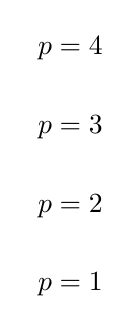
\begin{tikzpicture}
		\draw (0,-2) node[anchor=west] {$p=1$};
		\draw (0,-1) node[anchor=west] {$p=2$};
		\draw (0,0) node[anchor= west] {$p=3$};
		\draw (0,1) node[anchor= west] {$p=4$};
	\end{tikzpicture}
	\begin{tikzpicture}[line cap=round,line join=round,>=triangle 45,x=1cm,y=1cm]
		%\clip(-3.4905745922175466,-9.485443631543706) rectangle (8.35815993106314,2.189471744302653);
		\draw [line width=1pt] (2,-2)-- (6,-2);
		\draw [line width=1pt] (2,-1)-- (6,-1);
		\draw [line width=1pt] (2,0)-- (6,0);
		\draw [line width=1pt] (2,1)-- (6,1);
		\draw [line width=1pt] (4.6143253381220655,0) circle (6pt);
		\draw [line width=1pt] (3.4151309606738582,0) circle (6pt);
		\draw [line width=1pt] (3.4013471172549132,1) circle (6pt);
		\draw [line width=1pt] (4.6143253381220655,1) circle (6pt);
		\begin{scriptsize}
		\draw [fill=xdxdff] (3.4151309606738582,-2) circle (6pt);
		\draw [fill=xdxdff] (4.5867576512841755,-2) circle (6pt);
		\draw [fill=xdxdff] (3.3875632738359682,-1) circle (6pt);
		\draw [fill=xdxdff] (4.600541494703121,-1) circle (6pt);
		\end{scriptsize}
	\end{tikzpicture} 
	\begin{tikzpicture}[line cap=round,line join=round,>=triangle 45,x=1cm,y=1cm]
		%\clip(-3.4905745922175466,-9.485443631543706) rectangle (8.35815993106314,2.189471744302653);
		\draw [line width=1pt] (2,-2)-- (6,-2);
		\draw [line width=1pt] (2,-1)-- (6,-1);
		\draw [line width=1pt] (2,0)-- (6,0);
		\draw [line width=1pt] (2,1)-- (6,1);
		\draw [fill=xdxdff] (4.6143253381220655,0) circle (6pt);
		\draw [fill=xdxdff] (3.4151309606738582,0) circle (6pt);
		\draw [line width=1pt] (3.4013471172549132,1) circle (6pt);
		\draw [line width=1pt] (4.6143253381220655,1) circle (6pt);
		\begin{scriptsize}
		\draw [fill=xdxdff] (3.4151309606738582,-2) circle (6pt);
		\draw [fill=xdxdff] (4.5867576512841755,-2) circle (6pt);
		\draw [line width=1pt] (3.3875632738359682,-1) circle (6pt);
		\draw [line width=1pt] (4.600541494703121,-1) circle (6pt);
		\end{scriptsize}
	\end{tikzpicture} 
	\begin{tikzpicture}[line cap=round,line join=round,>=triangle 45,x=1cm,y=1cm]
		%\clip(-3.4905745922175466,-9.485443631543706) rectangle (8.35815993106314,2.189471744302653);
		\draw [line width=1pt] (2,-2)-- (6,-2);
		\draw [line width=1pt] (2,-1)-- (6,-1);
		\draw [line width=1pt] (2,0)-- (6,0);
		\draw [line width=1pt] (2,1)-- (6,1);
		\draw [line width=1pt] (4.6143253381220655,0) circle (6pt);
		\draw [fill=xdxdff] (3.4151309606738582,0) circle (6pt);
		\draw [line width=1pt] (3.4013471172549132,1) circle (6pt);
		\draw [line width=1pt] (4.6143253381220655,1) circle (6pt);
		\begin{scriptsize}
		\draw [line width=1pt] (3.4151309606738582,-1) circle (6pt);
		\draw [fill=xdxdff] (4.5867576512841755,-2) circle (6pt);
		\draw [fill=xdxdff] (3.3875632738359682,-2) circle (6pt);
		\draw [fill=xdxdff] (4.600541494703121,-1) circle (6pt);
		\end{scriptsize}
	\end{tikzpicture} 
	\caption{Illustration of the pairing model with $ 4 $ doubly degenerate single particle states and $ 4 $ particles. The Left shows all the particles are in the lowest-lying states. The middle figure shows a doubly excited state where no pairs are broken. The right figure shows a state with a singly excited particle where a pair is broken.}
	\label{fig:pairing-model}
\end{figure}


Without loss of generality, we set $ \xi=1 $ and vary the value of $ g $, the pairing strength. 
Consider the spin project operator 
\begin{align}
	\label{eq:spin-proj}
	\hat{S}_z & =\frac{1}{2} \sum_{p, \sigma} \sigma \hat{a}_{p \sigma}^{\dagger} \hat{a}_{p \sigma}, \\ 
	\hat{S}^2 & =\hat{S}_z^2+\frac{1}{2}\left(\hat{S}_{+} \hat{S}_{-}+\hat{S}_{-} \hat{S}_{+}\right), \\ 
	\hat{S}_{\pm} & =\sum_p \hat{a}_{p \pm}^{\dagger} \hat{a}_{p \mp}.
\end{align}
The pair creation and annihilation operators are defined as 
\begin{equation}
	\label{eq:pairingCreAnn}
	\hat{P}_p^{+}=\hat{a}_{p+}^{\dagger} \hat{a}_{p-}^{\dagger}, \quad \hat{P}_p^{-}=\hat{a}_{p-} \hat{a}_{p+}.
\end{equation}
The pairing Hamiltonian can be rewritten as 

\begin{equation}
	\label{eq:pairing-inP}
	\hat{H}=\sum_{p \sigma}(p-1) a_{p \sigma}^{\dagger} a_{p \sigma}-\frac{1}{2} g \sum_{p q} \hat{P}_p^{+} \hat{P}_q^{-}.
\end{equation}
To set up the matrix Hamiltonian for where no pair is broken we need to set up the basis for the system. We include all possible combinations for the $ 4 $ particles to occupy the $ 4 $ doubly degenerate states without breaking any pairs as the basis. Such that
\begin{equation}
	\label{eq:pairing-basis}
	\begin{aligned}
		\ket{\phi_0} &= \ket{1_+,1_-,2_+,2_=} = \hat a_{2+}^{\dagger} \hat a_{2-}^{\dagger} \hat a_{1+}^{\dagger} \hat a_{1-}^{\dagger} = \hat P_{2}^{+} \hat P_{1}^{+} \ket{0}  \\
		\ket{\phi_1} &= \ket{1_+,1_-,3_+,3_-} = \hat P_{3}^{+} \hat P_{1}^{+} \ket{0} \\
		\ket{\phi_2} &= \ket{1_+,1_-,4_+,4_-} = \hat P_{4}^{+} \hat P_{1}^{+} \ket{0} \\
		\ket{\phi_3} &= \ket{2_+,2_-,3_+,3_-} = \hat P_{3}^{+} \hat P_{2}^{+} \ket{0} \\
		\ket{\phi_4} &= \ket{2_+,2_-,4_+,4_-}  = \hat P_{4}^{+} \hat P_{2}^{+} \ket{0} \\
		\ket{\phi_5} &= \ket{3_+,3_-,4_+,4_-} = \hat P_{4}^{+} \hat P_{3}^{+} \ket{0}.
	\end{aligned}
\end{equation}
Let 
\[ \left|\Phi_0\right\rangle=\left(\begin{array}{l}
1 \\
0 \\
0 \\
0 \\
0 \\
0
\end{array}\right), \quad\left|\Phi_1\right\rangle=\left(\begin{array}{l}
0 \\
1 \\
0 \\
0 \\
0 \\
0
\end{array}\right), \quad \cdots \quad\left|\Phi_5\right\rangle=\left(\begin{array}{l}
0 \\
0 \\
0 \\
0 \\
0 \\
1
\end{array}\right), \] 
be the basis for the system, and compute the matrix element $ \braket{\phi_i|\hat H|\phi_j} $ using Equation~\eqref{eq:pairingCreAnn}. We obtain that the matrix representation of the Hamiltonian
\begin{equation}
    \label{eq:pairing-mat}
	\hat{H}= \begin{pmatrix} 
	2-g & -g / 2 & -g / 2 & -g / 2 & -g / 2 & 0 \\
	-g / 2 & 4-g & -g / 2 & -g / 2 & 0 & -g / 2 \\
	-g / 2 & -g / 2 & 6-g & 0 & -g / 2 & -g / 2 \\
	-g / 2 & -g / 2 & 0 & 6-g & -g / 2 & -g / 2 \\
	-g / 2 & 0 & -g / 2 & -g / 2 & 8-g & -g / 2 \\
	0 & -g / 2 & -g / 2 & -g / 2 & -g / 2 & 10-g
	 \end{pmatrix}.
\end{equation}
We will encode this Hamiltonian using Pauli Decomposition into qubit Hamiltonian for the VQEs. The Hamiltonian has $ 18 $ terms.

The qubit Hamiltonian is given in Table~\ref{tab:pairing-qh}.

\begin{table}[ht]
    \centering
    \begin{tabular}{cc}
        \toprule
        \textbf{Pauli String} & \textbf{Coefficient} \\ 
        \midrule
        III & 28.5 \\ 
        IIX & -0.25 \\ 
        IIZ & -0.5 \\ 
        IXI & -0.25 \\ 
        IXX & -0.25 \\ 
        IZI & -23.5 \\ 
        IZX & -0.25 \\ 
        IZZ & -0.5 \\ 
        XII & -0.25 \\ 
        XXI & -0.25 \\ 
        XXX & -0.25 \\ 
        XZI & -0.25 \\ 
        YYI & -0.25 \\ 
        YYX & -0.25 \\ 
        ZII & -25 \\ 
        ZXI & -0.25 \\ 
        ZXX & -0.25 \\ 
        ZZI & 22 \\ 
        \bottomrule
    \end{tabular}
    \caption{Pauli strings and their coefficients.}
    \label{tab:pairing-qh}
\end{table}


\section{Deuteron Model}
\label{sec:deutron_model}

The deuteron model is a bound state of a proton and a neutron, which is surprisingly stable since neutrons are famously not~\cite{mit_deuteron}. We follow the derivation of the deuteron Hamiltonian as~\cite{Dumitrescu2018, Binder2016, Bansal2017} for our simulation, where a discrete variable representation in the harmonic oscillator basis is used. The Hamiltonian is given as
\begin{equation}
    \label{eq:deuteron-hamiltonian}
	H_N=\sum_{n, n^{\prime}=0}^{N-1}\left\langle n^{\prime}|(T+V)| n\right\rangle a_{n^{\prime}}^{\dagger} a_n.
\end{equation}
where $ n $ is the harmonic oscillator quantum number, $ a_n^\dagger, a_n $ are the creation and annihilation operators for the deuteron in the harmonic oscillator s-wave state $\ket{n} $, $ T $ is the kinetic energy operator and $ V $ is the potential energy operator. The kinetic energy operator $ T $ and potential energy operator $ V $ are given by 

\begin{equation}
	\begin{aligned}
	\left\langle n^{\prime}|T| n\right\rangle= & \frac{\hbar \omega}{2}\left[(2 n+3 / 2) \delta_n^{n^{\prime}}-\sqrt{n(n+1 / 2)} \delta_n^{n^{\prime}+1}\right. \left.-\sqrt{(n+1)(n+3 / 2)} \delta_n^{n^{\prime}-1}\right], \\
	\left\langle n^{\prime}|V| n\right\rangle= & V_0 \delta_n^0 \delta_n^{n^{\prime}},
	\end{aligned}
\end{equation}
where $V_0 = -5.68658111 $ MeV and $ \hbar \omega = 7 $ MeV.

The Jordan-Wigner transform was used in \cite{Dumitrescu2018} to map the Deuteron Hamiltonian to qubit Hamiltonian. Glancing through Equation~\eqref{eq:deuteron-hamiltonian} yields that it does not have any two-body term, which means transforming it with Jordan-Wigner transformation is wasteful. However, rewriting it into a Hamiltonian matrix and then using the Pauli decomposition saves the number of qubits required to represent the system. This is a huge advantage for any algorithm running on NISQ devices, especially since the basis dimension $ N $ can increase indefinitely. Since we are able to save on the number of qubits we will push the basis dimension $ N $ to higher values than the $ N=3 $ in the original paper.

